\documentclass{standalone}
\usepackage{tikz}
\usepackage{pgfplots}
\pgfplotsset{compat=newest}

\begin{document}
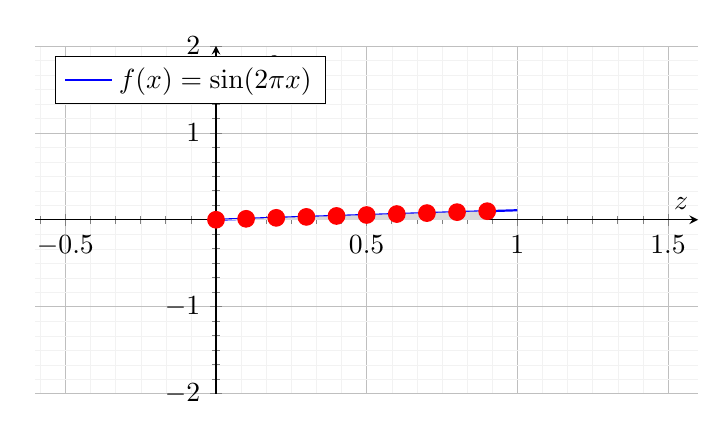
\begin{tikzpicture}
\begin{axis}[
    axis lines = middle,
    xlabel = \(z\),
    ylabel = {\(f(x^{2})\)},
    ymin=-1.5, ymax=1.5,
    xmin=-0.1, xmax=1.1,
    width=10cm,
    height=6cm,
    grid=both,
    grid style={line width=.1pt, draw=gray!10},
    major grid style={line width=.2pt,draw=gray!50},
    minor tick num=5,
    enlargelimits={abs=0.5},
    samples=100,
    domain=0:1,
    legend pos=north west,
]

% 绘制函数曲线
\addplot [domain=0:1, samples=100, color=blue, thick] {sin(2*pi*x)};
\addlegendentry{\(f(x) = \sin(2\pi x)\)}

% 绘制网格点
\foreach \x in {0, 0.1, ..., 1} {
    \addplot[mark=*, mark size=3, color=red] coordinates {(\x, {sin(2*pi*\x)})};
}

% 绘制积分区域
\foreach \x in {0, 0.1, ..., 0.9} {
    \addplot [fill=gray!30, draw=none, domain=\x:{\x+0.1}] {sin(2*pi*x)} \closedcycle;
}

\end{axis}
\end{tikzpicture}
\end{document}